\documentclass[letterpaper]{book}
\usepackage{makeidx}
\usepackage{graphicx}
\usepackage{multicol}
\usepackage{float}
\usepackage{listings}
\usepackage{color}
\usepackage{textcomp}
\usepackage{alltt}
\usepackage{times}
\usepackage{ifpdf}
\ifpdf
\usepackage[pdftex,
            pagebackref=true,
            colorlinks=true,
            linkcolor=blue,
            unicode
           ]{hyperref}
\else
\usepackage[ps2pdf,
            pagebackref=true,
            colorlinks=true,
            linkcolor=blue,
            unicode
           ]{hyperref}
\usepackage{pspicture}
\fi
\usepackage[utf8]{inputenc}
\usepackage{doxygen}
\lstset{language=C++,inputencoding=utf8,basicstyle=\footnotesize,breaklines=true,breakatwhitespace=true,tabsize=8,numbers=left }
\makeindex
\setcounter{tocdepth}{3}
\renewcommand{\footrulewidth}{0.4pt}
\begin{document}
\hypersetup{pageanchor=false}
\begin{titlepage}
\vspace*{7cm}
\begin{center}
{\Large WIRemoting \\[1ex]\large 1.0 }\\
\vspace*{1cm}
{\large Generated by Doxygen 1.6.1}\\
\vspace*{0.5cm}
{\small Thu Dec 3 21:15:04 2009}\\
\end{center}
\end{titlepage}
\clearemptydoublepage
\pagenumbering{roman}
\tableofcontents
\clearemptydoublepage
\pagenumbering{arabic}
\hypersetup{pageanchor=true}
\chapter{Class Index}
\section{Class Hierarchy}
This inheritance list is sorted roughly, but not completely, alphabetically:\begin{DoxyCompactList}
\item \contentsline{section}{ASIHTTPRequest}{\pageref{interface_a_s_i_h_t_t_p_request}}{}
\begin{DoxyCompactList}
\item \contentsline{section}{ASIFormDataRequest}{\pageref{interface_a_s_i_form_data_request}}{}
\item \contentsline{section}{ASIS3Request}{\pageref{interface_a_s_i_s3_request}}{}
\begin{DoxyCompactList}
\item \contentsline{section}{ASIS3ListRequest}{\pageref{interface_a_s_i_s3_list_request}}{}
\end{DoxyCompactList}
\end{DoxyCompactList}
\item \contentsline{section}{ASINetworkQueue}{\pageref{interface_a_s_i_network_queue}}{}
\item \contentsline{section}{NSObject}{\pageref{class_n_s_object}}{}
\begin{DoxyCompactList}
\item \contentsline{section}{ASIAuthenticationDialog}{\pageref{interface_a_s_i_authentication_dialog}}{}
\item \contentsline{section}{ASIInputStream}{\pageref{interface_a_s_i_input_stream}}{}
\item \contentsline{section}{ASIS3BucketObject}{\pageref{interface_a_s_i_s3_bucket_object}}{}
\item \contentsline{section}{Mock}{\pageref{interface_mock}}{}
\item \contentsline{section}{MockProtocol}{\pageref{interface_mock_protocol}}{}
\item \contentsline{section}{MockProtocol2}{\pageref{interface_mock_protocol2}}{}
\item \contentsline{section}{MockProtocolShouldSend}{\pageref{interface_mock_protocol_should_send}}{}
\item \contentsline{section}{MockSessionProtocol}{\pageref{interface_mock_session_protocol}}{}
\item \contentsline{section}{Reachability}{\pageref{interface_reachability}}{}
\item \contentsline{section}{ReachabilityQuery}{\pageref{interface_reachability_query}}{}
\item \contentsline{section}{RMCall}{\pageref{interface_r_m_call}}{}
\item \contentsline{section}{RMResponse}{\pageref{interface_r_m_response}}{}
\item \contentsline{section}{RMSession}{\pageref{interface_r_m_session}}{}
\item \contentsline{section}{RMStatus}{\pageref{interface_r_m_status}}{}
\item \contentsline{section}{SBJsonBase}{\pageref{interface_s_b_json_base}}{}
\begin{DoxyCompactList}
\item \contentsline{section}{SBJSON}{\pageref{interface_s_b_j_s_o_n}}{}
\item \contentsline{section}{SBJsonParser}{\pageref{interface_s_b_json_parser}}{}
\item \contentsline{section}{SBJsonWriter}{\pageref{interface_s_b_json_writer}}{}
\end{DoxyCompactList}
\end{DoxyCompactList}
\item \contentsline{section}{NSString}{\pageref{class_n_s_string}}{}
\item \contentsline{section}{$<$RMAuthenticator$>$}{\pageref{protocol_r_m_authenticator-p}}{}
\begin{DoxyCompactList}
\item \contentsline{section}{RMSessionTests}{\pageref{interface_r_m_session_tests}}{}
\end{DoxyCompactList}
\item \contentsline{section}{$<$RMCallProtocol$>$}{\pageref{protocol_r_m_call_protocol-p}}{}
\begin{DoxyCompactList}
\item \contentsline{section}{MockProtocol}{\pageref{interface_mock_protocol}}{}
\item \contentsline{section}{MockProtocol2}{\pageref{interface_mock_protocol2}}{}
\item \contentsline{section}{MockProtocolShouldSend}{\pageref{interface_mock_protocol_should_send}}{}
\item \contentsline{section}{MockSessionProtocol}{\pageref{interface_mock_session_protocol}}{}
\item \contentsline{section}{RMSessionTests}{\pageref{interface_r_m_session_tests}}{}
\end{DoxyCompactList}
\item \contentsline{section}{RMCallTests}{\pageref{interface_r_m_call_tests}}{}
\item \contentsline{section}{$<$RMResultDelegate$>$}{\pageref{protocol_r_m_result_delegate-p}}{}
\begin{DoxyCompactList}
\item \contentsline{section}{Mock}{\pageref{interface_mock}}{}
\item \contentsline{section}{RMSession}{\pageref{interface_r_m_session}}{}
\item \contentsline{section}{RMSessionTests}{\pageref{interface_r_m_session_tests}}{}
\end{DoxyCompactList}
\item \contentsline{section}{$<$SBJsonParser$>$}{\pageref{protocol_s_b_json_parser-p}}{}
\begin{DoxyCompactList}
\item \contentsline{section}{SBJSON}{\pageref{interface_s_b_j_s_o_n}}{}
\item \contentsline{section}{SBJsonParser}{\pageref{interface_s_b_json_parser}}{}
\end{DoxyCompactList}
\item \contentsline{section}{$<$SBJsonWriter$>$}{\pageref{protocol_s_b_json_writer-p}}{}
\begin{DoxyCompactList}
\item \contentsline{section}{SBJSON}{\pageref{interface_s_b_j_s_o_n}}{}
\item \contentsline{section}{SBJsonWriter}{\pageref{interface_s_b_json_writer}}{}
\end{DoxyCompactList}
\end{DoxyCompactList}

\chapter{Class Index}
\section{Class List}
Here are the classes, structs, unions and interfaces with brief descriptions:\begin{DoxyCompactList}
\item\contentsline{section}{\hyperlink{interface_mock_protocol}{MockProtocol} }{\pageref{interface_mock_protocol}}{}
\item\contentsline{section}{\hyperlink{interface_mock_protocol2}{MockProtocol2} }{\pageref{interface_mock_protocol2}}{}
\item\contentsline{section}{\hyperlink{interface_mock_protocol_should_send}{MockProtocolShouldSend} }{\pageref{interface_mock_protocol_should_send}}{}
\item\contentsline{section}{\hyperlink{interface_mock_session_protocol}{MockSessionProtocol} }{\pageref{interface_mock_session_protocol}}{}
\item\contentsline{section}{\hyperlink{interface_moodle}{Moodle} }{\pageref{interface_moodle}}{}
\item\contentsline{section}{\hyperlink{interface_moodle_authenticator}{MoodleAuthenticator} }{\pageref{interface_moodle_authenticator}}{}
\item\contentsline{section}{\hyperlink{interface_moodle_call_protocol}{MoodleCallProtocol} }{\pageref{interface_moodle_call_protocol}}{}
\item\contentsline{section}{\hyperlink{interface_moodle_result}{MoodleResult} }{\pageref{interface_moodle_result}}{}
\item\contentsline{section}{\hyperlink{protocol_r_m_authenticator-p}{$<$RMAuthenticator$>$} (The authentication provider )}{\pageref{protocol_r_m_authenticator-p}}{}
\item\contentsline{section}{\hyperlink{interface_r_m_call}{RMCall} (Handles calls in WIRemoting framework )}{\pageref{interface_r_m_call}}{}
\item\contentsline{section}{\hyperlink{protocol_r_m_call_protocol-p}{$<$RMCallProtocol$>$} (Provides call protocol interface/implementation )}{\pageref{protocol_r_m_call_protocol-p}}{}
\item\contentsline{section}{\hyperlink{interface_r_m_call_tests}{RMCallTests} }{\pageref{interface_r_m_call_tests}}{}
\item\contentsline{section}{\hyperlink{interface_r_m_response}{RMResponse} (Handles call responses in WIRemoting framework )}{\pageref{interface_r_m_response}}{}
\item\contentsline{section}{\hyperlink{protocol_r_m_result_delegate-p}{$<$RMResultDelegate$>$} (Handles call results in WIRemoting framework )}{\pageref{protocol_r_m_result_delegate-p}}{}
\item\contentsline{section}{\hyperlink{interface_r_m_result_delegate_wrapper}{RMResultDelegateWrapper} }{\pageref{interface_r_m_result_delegate_wrapper}}{}
\item\contentsline{section}{\hyperlink{interface_r_m_session}{RMSession} (Handles sessions in WIRemoting framework )}{\pageref{interface_r_m_session}}{}
\item\contentsline{section}{\hyperlink{interface_r_m_session_tests}{RMSessionTests} }{\pageref{interface_r_m_session_tests}}{}
\item\contentsline{section}{\hyperlink{interface_r_m_status}{RMStatus} }{\pageref{interface_r_m_status}}{}
\end{DoxyCompactList}

\chapter{Class Documentation}
\hypertarget{interface_mock}{
\section{Mock Class Reference}
\label{interface_mock}\index{Mock@{Mock}}
}
Inheritance diagram for Mock::\begin{figure}[H]
\begin{center}
\leavevmode
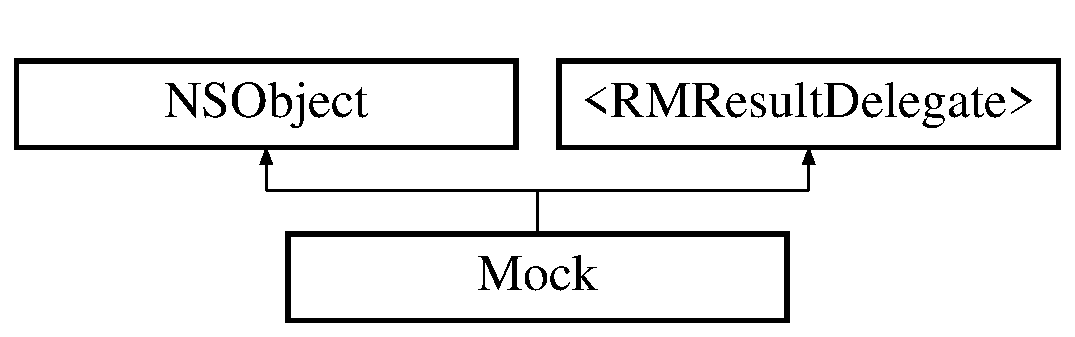
\includegraphics[height=2cm]{interface_mock}
\end{center}
\end{figure}
\subsection*{Public Member Functions}
\begin{DoxyCompactItemize}
\item 
\hypertarget{interface_mock_a24935b458f7a6a2aa01b28e9c5f81b63}{
(id) -\/ {\bfseries initWithObject:finished:failed:}}
\label{interface_mock_a24935b458f7a6a2aa01b28e9c5f81b63}

\item 
(void) -\/ \hyperlink{interface_mock_ab15e59579bf7b5c5de900d28374062b7}{finished:}
\begin{DoxyCompactList}\small\item\em An event fired when the call successfully finishes. \item\end{DoxyCompactList}\item 
(void) -\/ \hyperlink{interface_mock_ae57e780c8ddcf5c4c79af12c54d58cff}{failed:error:}
\begin{DoxyCompactList}\small\item\em An event fired when the call fails. \item\end{DoxyCompactList}\end{DoxyCompactItemize}
\subsection*{Protected Attributes}
\begin{DoxyCompactItemize}
\item 
\hypertarget{interface_mock_acd44dbbfc0cf1442f66471cdab70f642}{
id {\bfseries object}}
\label{interface_mock_acd44dbbfc0cf1442f66471cdab70f642}

\item 
\hypertarget{interface_mock_a28044b61b39281421caafdb81ef258cf}{
SEL {\bfseries finished}}
\label{interface_mock_a28044b61b39281421caafdb81ef258cf}

\item 
\hypertarget{interface_mock_a25af3f8adbc951c4ea3b6b4a1e5687d3}{
SEL {\bfseries failed}}
\label{interface_mock_a25af3f8adbc951c4ea3b6b4a1e5687d3}

\end{DoxyCompactItemize}


\subsection{Detailed Description}


Definition at line 14 of file Mock.h.

\subsection{Member Function Documentation}
\hypertarget{interface_mock_ab15e59579bf7b5c5de900d28374062b7}{
\index{Mock@{Mock}!finished:@{finished:}}
\index{finished:@{finished:}!Mock@{Mock}}
\subsubsection[{finished:}]{\setlength{\rightskip}{0pt plus 5cm}-\/ (void) finished: ({\bf RMResponse} $\ast$) {\em response}}}
\label{interface_mock_ab15e59579bf7b5c5de900d28374062b7}


An event fired when the call successfully finishes. 
\begin{DoxyParams}{Parameters}
\item[{\em response}]A response object from the remote call. \end{DoxyParams}


Reimplemented from \hyperlink{protocol_r_m_result_delegate-p_a965fe7cc4e150bb6ecf7cbb02b9c7248}{$<$RMResultDelegate$>$}.

Definition at line 27 of file Mock.m.\hypertarget{interface_mock_ae57e780c8ddcf5c4c79af12c54d58cff}{
\index{Mock@{Mock}!failed:error:@{failed:error:}}
\index{failed:error:@{failed:error:}!Mock@{Mock}}
\subsubsection[{failed:error:}]{\setlength{\rightskip}{0pt plus 5cm}-\/ (void) failed: ({\bf RMResponse} $\ast$) {\em response}\/ error: (NSError $\ast$) {\em error}}}
\label{interface_mock_ae57e780c8ddcf5c4c79af12c54d58cff}


An event fired when the call fails. 
\begin{DoxyParams}{Parameters}
\item[{\em response}]A response object from the remote peer. \item[{\em error}]An error object from the remote peer. \end{DoxyParams}


Reimplemented from \hyperlink{protocol_r_m_result_delegate-p_a3521cd9555449b32aabdb759d2dadce5}{$<$RMResultDelegate$>$}.

Definition at line 33 of file Mock.m.

The documentation for this class was generated from the following files:\begin{DoxyCompactItemize}
\item 
/Users/yxh/Code/XCode/WIRemoting/Tests/UnitTests/Mock.h\item 
/Users/yxh/Code/XCode/WIRemoting/Tests/UnitTests/Mock.m\end{DoxyCompactItemize}

\hypertarget{interface_mock_protocol}{
\section{MockProtocol Class Reference}
\label{interface_mock_protocol}\index{MockProtocol@{MockProtocol}}
}
Inheritance diagram for MockProtocol::\begin{figure}[H]
\begin{center}
\leavevmode
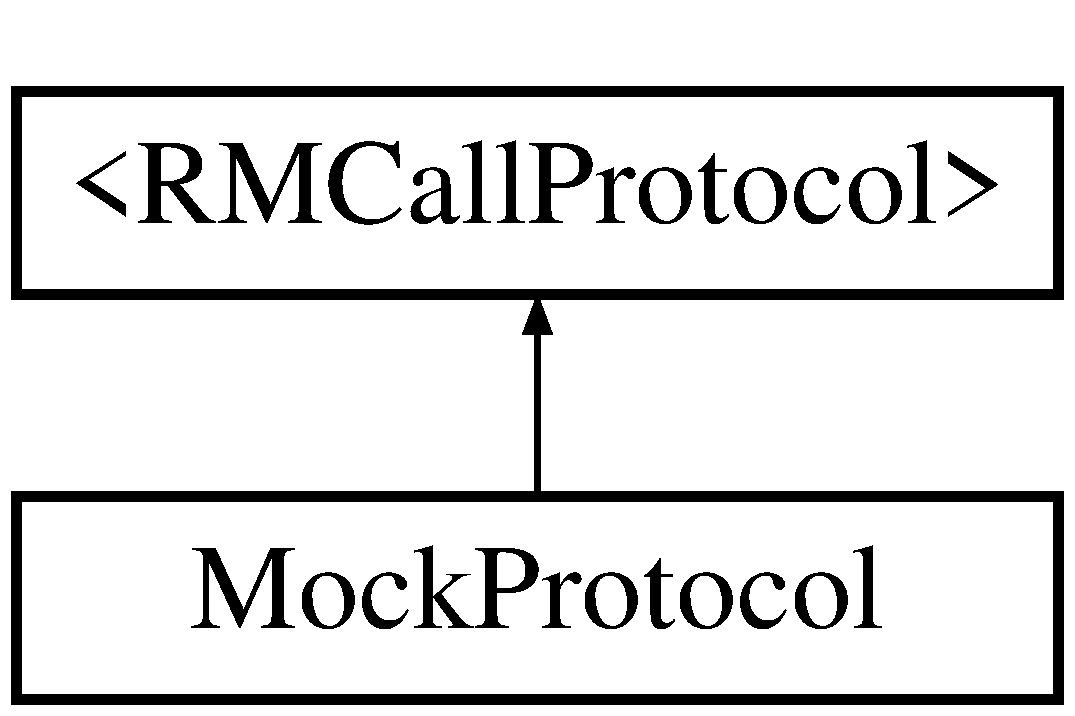
\includegraphics[height=2cm]{interface_mock_protocol}
\end{center}
\end{figure}
\subsection*{Public Member Functions}
\begin{DoxyCompactItemize}
\item 
\hypertarget{interface_mock_protocol_af1dbb6f419ecd6fe8cb3f73e2dee276b}{
(void) -\/ {\bfseries adjustRequest:method:arguments:}}
\label{interface_mock_protocol_af1dbb6f419ecd6fe8cb3f73e2dee276b}

\end{DoxyCompactItemize}


\subsection{Detailed Description}


Definition at line 12 of file MockProtocol.h.

The documentation for this class was generated from the following file:\begin{DoxyCompactItemize}
\item 
/Users/yxh/Code/XCode/WIRemoting/Source/Tests/UnitTests/MockProtocol.h\end{DoxyCompactItemize}

\hypertarget{interface_mock_protocol2}{
\section{MockProtocol2 Class Reference}
\label{interface_mock_protocol2}\index{MockProtocol2@{MockProtocol2}}
}
Inheritance diagram for MockProtocol2::\begin{figure}[H]
\begin{center}
\leavevmode
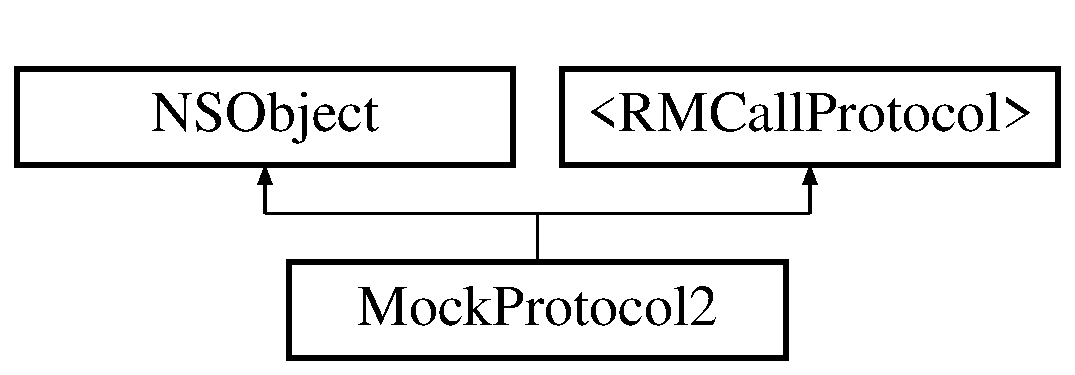
\includegraphics[height=2cm]{interface_mock_protocol2}
\end{center}
\end{figure}


\subsection{Detailed Description}


Definition at line 12 of file MockProtocol2.h.

The documentation for this class was generated from the following file:\begin{DoxyCompactItemize}
\item 
/Users/yxh/Code/XCode/WIRemoting/Tests/UnitTests/MockProtocol2.h\end{DoxyCompactItemize}

\hypertarget{interface_mock_protocol_should_send}{
\section{MockProtocolShouldSend Class Reference}
\label{interface_mock_protocol_should_send}\index{MockProtocolShouldSend@{MockProtocolShouldSend}}
}
Inheritance diagram for MockProtocolShouldSend::\begin{figure}[H]
\begin{center}
\leavevmode
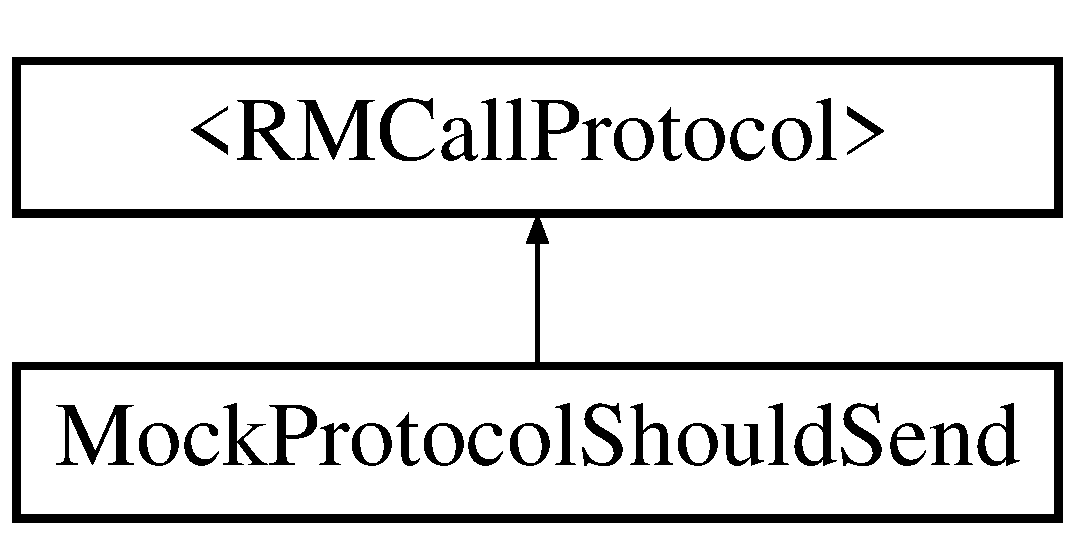
\includegraphics[height=2cm]{interface_mock_protocol_should_send}
\end{center}
\end{figure}


\subsection{Detailed Description}


Definition at line 13 of file MockProtocolShouldSend.h.

The documentation for this class was generated from the following file:\begin{DoxyCompactItemize}
\item 
/Users/yxh/Code/XCode/WIRemoting/Source/Tests/UnitTests/MockProtocolShouldSend.h\end{DoxyCompactItemize}

\hypertarget{interface_mock_session_protocol}{
\section{MockSessionProtocol Class Reference}
\label{interface_mock_session_protocol}\index{MockSessionProtocol@{MockSessionProtocol}}
}
Inheritance diagram for MockSessionProtocol::\begin{figure}[H]
\begin{center}
\leavevmode
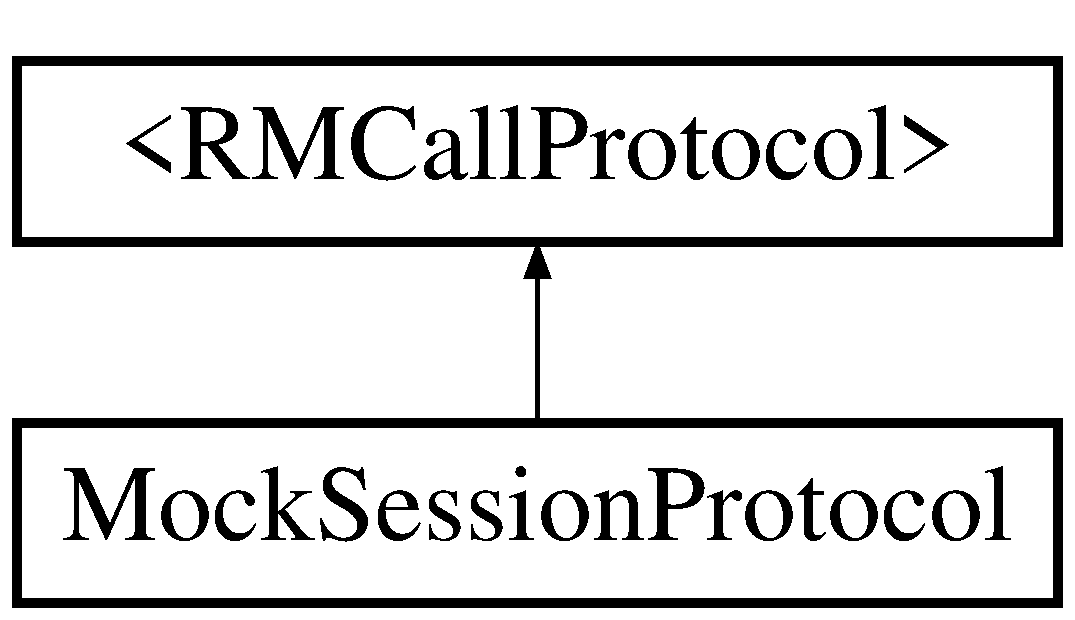
\includegraphics[height=2cm]{interface_mock_session_protocol}
\end{center}
\end{figure}


\subsection{Detailed Description}


Definition at line 13 of file MockSessionProtocol.h.

The documentation for this class was generated from the following file:\begin{DoxyCompactItemize}
\item 
/Users/yxh/Code/XCode/WIRemoting/Tests/UnitTests/MockSessionProtocol.h\end{DoxyCompactItemize}

\hypertarget{protocol_r_m_authenticator-p}{
\section{$<$RMAuthenticator$>$ Protocol Reference}
\label{protocol_r_m_authenticator-p}\index{RMAuthenticator-\/p@{RMAuthenticator-\/p}}
}


The authentication provider.  


{\ttfamily \#import $<$RMSession.h$>$}Inheritance diagram for $<$RMAuthenticator$>$::\begin{figure}[H]
\begin{center}
\leavevmode
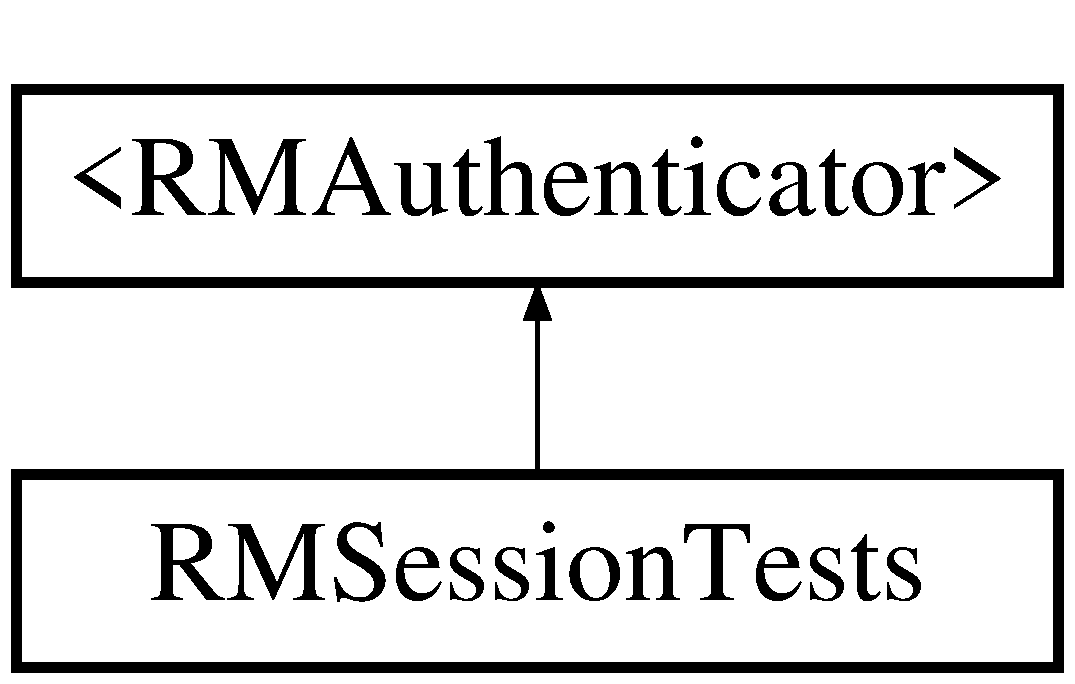
\includegraphics[height=2cm]{protocol_r_m_authenticator-p}
\end{center}
\end{figure}
\subsection*{Public Member Functions}
\begin{DoxyCompactItemize}
\item 
(void) -\/ \hyperlink{protocol_r_m_authenticator-p_a89800622f7067e082cbb6665f51d44c8}{authenticateWithCall:delegate:}
\begin{DoxyCompactList}\small\item\em Authenticate the session with a call object. \item\end{DoxyCompactList}\item 
(id$<$ \hyperlink{protocol_r_m_call_protocol-p}{RMCallProtocol} $>$) -\/ \hyperlink{protocol_r_m_authenticator-p_a1a8ee1ab6eb4014dd3783e096173f000}{callProtocol}
\begin{DoxyCompactList}\small\item\em A call protocol to handle session credentials for subsequent calls. \item\end{DoxyCompactList}\item 
(BOOL) -\/ \hyperlink{protocol_r_m_authenticator-p_adf5dc80e89981e86b61d1720ad441c79}{authenticateResponseString:}
\begin{DoxyCompactList}\small\item\em Check the responseString if the response is authenticated. \item\end{DoxyCompactList}\item 
(BOOL) -\/ \hyperlink{protocol_r_m_authenticator-p_aa82480a76b720c6497425661de692eea}{authenticateResponseData:}
\begin{DoxyCompactList}\small\item\em Check the responseData if the response is authenticated. \item\end{DoxyCompactList}\end{DoxyCompactItemize}


\subsection{Detailed Description}
The authentication provider. 

Definition at line 21 of file RMSession.h.

\subsection{Member Function Documentation}
\hypertarget{protocol_r_m_authenticator-p_a89800622f7067e082cbb6665f51d44c8}{
\index{RMAuthenticator-\/p@{RMAuthenticator-\/p}!authenticateWithCall:delegate:@{authenticateWithCall:delegate:}}
\index{authenticateWithCall:delegate:@{authenticateWithCall:delegate:}!RMAuthenticator-p@{RMAuthenticator-\/p}}
\subsubsection[{authenticateWithCall:delegate:}]{\setlength{\rightskip}{0pt plus 5cm}-\/ (void) authenticateWithCall: ({\bf RMCall} $\ast$) {\em call}\/ delegate: (id$<$ {\bf RMResultDelegate} $>$) {\em delegate}\hspace{0.3cm}{\ttfamily  \mbox{[}required\mbox{]}}}}
\label{protocol_r_m_authenticator-p_a89800622f7067e082cbb6665f51d44c8}


Authenticate the session with a call object. 
\begin{DoxyParams}{Parameters}
\item[{\em call}]a \hyperlink{interface_r_m_call}{RMCall} object. \item[{\em delegate}]a RMSessionDelegate. \end{DoxyParams}
\hypertarget{protocol_r_m_authenticator-p_a1a8ee1ab6eb4014dd3783e096173f000}{
\index{RMAuthenticator-\/p@{RMAuthenticator-\/p}!callProtocol@{callProtocol}}
\index{callProtocol@{callProtocol}!RMAuthenticator-p@{RMAuthenticator-\/p}}
\subsubsection[{callProtocol}]{\setlength{\rightskip}{0pt plus 5cm}-\/ (id$<${\bf RMCallProtocol}$>$) callProtocol \hspace{0.3cm}{\ttfamily  \mbox{[}required\mbox{]}}}}
\label{protocol_r_m_authenticator-p_a1a8ee1ab6eb4014dd3783e096173f000}


A call protocol to handle session credentials for subsequent calls. \begin{DoxyReturn}{Returns}
An object implementing \hyperlink{protocol_r_m_call_protocol-p}{RMCallProtocol}. 
\end{DoxyReturn}
\hypertarget{protocol_r_m_authenticator-p_adf5dc80e89981e86b61d1720ad441c79}{
\index{RMAuthenticator-\/p@{RMAuthenticator-\/p}!authenticateResponseString:@{authenticateResponseString:}}
\index{authenticateResponseString:@{authenticateResponseString:}!RMAuthenticator-p@{RMAuthenticator-\/p}}
\subsubsection[{authenticateResponseString:}]{\setlength{\rightskip}{0pt plus 5cm}-\/ (BOOL) authenticateResponseString: (NSString $\ast$) {\em responseString}\hspace{0.3cm}{\ttfamily  \mbox{[}optional\mbox{]}}}}
\label{protocol_r_m_authenticator-p_adf5dc80e89981e86b61d1720ad441c79}


Check the responseString if the response is authenticated. 
\begin{DoxyParams}{Parameters}
\item[{\em responseString}]\end{DoxyParams}
\begin{DoxyReturn}{Returns}
true if the session is authenticated 
\end{DoxyReturn}
\hypertarget{protocol_r_m_authenticator-p_aa82480a76b720c6497425661de692eea}{
\index{RMAuthenticator-\/p@{RMAuthenticator-\/p}!authenticateResponseData:@{authenticateResponseData:}}
\index{authenticateResponseData:@{authenticateResponseData:}!RMAuthenticator-p@{RMAuthenticator-\/p}}
\subsubsection[{authenticateResponseData:}]{\setlength{\rightskip}{0pt plus 5cm}-\/ (BOOL) authenticateResponseData: (NSData $\ast$) {\em responseData}\hspace{0.3cm}{\ttfamily  \mbox{[}optional\mbox{]}}}}
\label{protocol_r_m_authenticator-p_aa82480a76b720c6497425661de692eea}


Check the responseData if the response is authenticated. 
\begin{DoxyParams}{Parameters}
\item[{\em responseData}]\end{DoxyParams}
\begin{DoxyReturn}{Returns}
true if the session is authenticated 
\end{DoxyReturn}


The documentation for this protocol was generated from the following file:\begin{DoxyCompactItemize}
\item 
/Users/yxh/Code/XCode/WIRemoting/Source/Classes/RMSession.h\end{DoxyCompactItemize}

\hypertarget{interface_r_m_call}{
\section{RMCall Class Reference}
\label{interface_r_m_call}\index{RMCall@{RMCall}}
}


Handles calls in WIRemoting framework.  


{\ttfamily \#import $<$RMCall.h$>$}Inheritance diagram for RMCall::\begin{figure}[H]
\begin{center}
\leavevmode
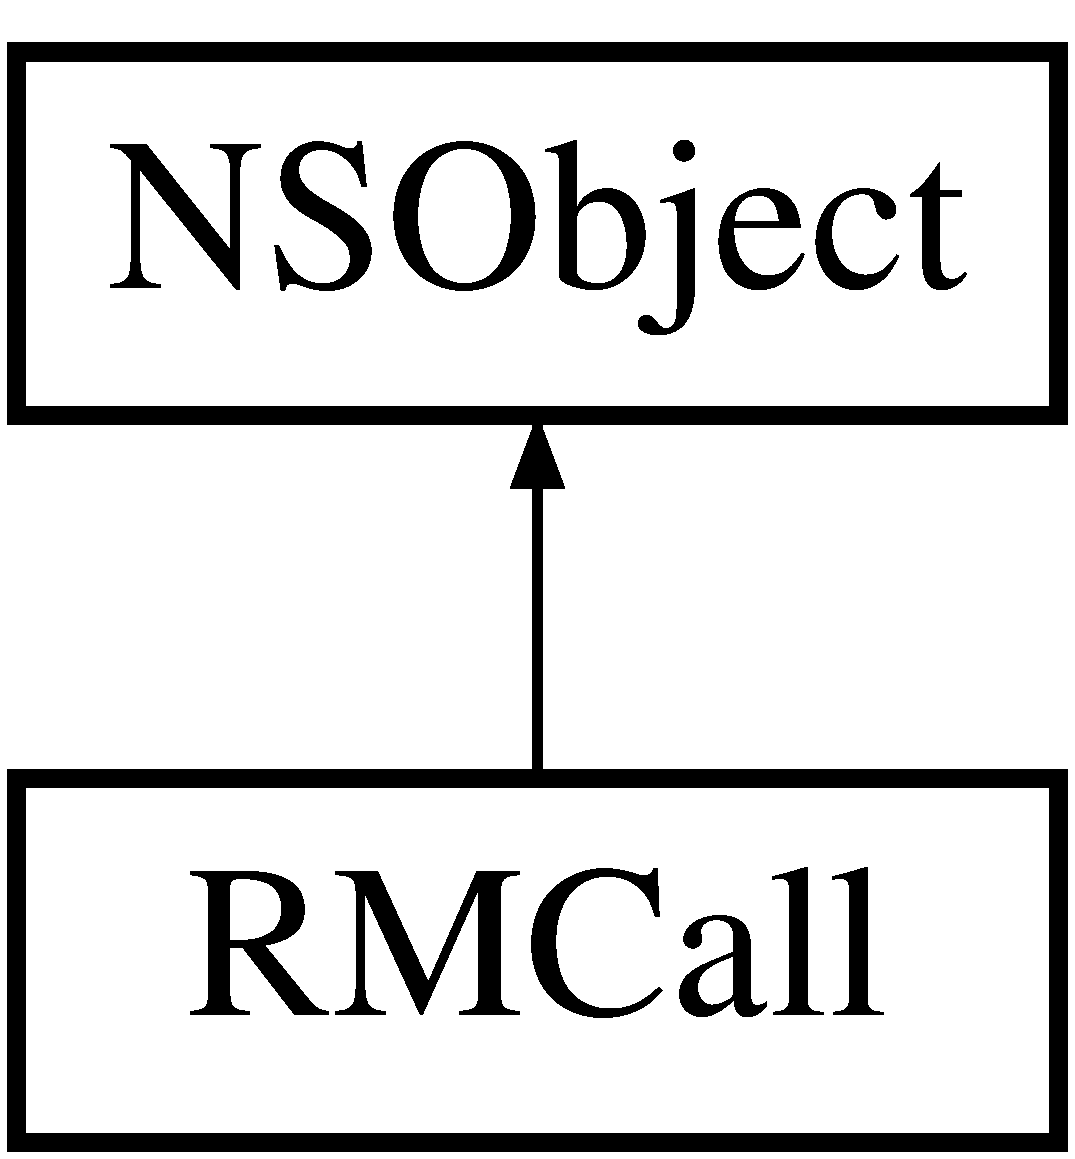
\includegraphics[height=2cm]{interface_r_m_call}
\end{center}
\end{figure}
\subsection*{Public Member Functions}
\begin{DoxyCompactItemize}
\item 
(id) -\/ \hyperlink{interface_r_m_call_a64f1e76758d2d473859064c5b0c6c75d}{initWithProtocol:}
\begin{DoxyCompactList}\small\item\em Initiatize the call with a call protocol. \item\end{DoxyCompactList}\item 
(BOOL) -\/ \hyperlink{interface_r_m_call_a85bb3ac47600a313105a6f94c9ab7ec3}{call:arguments:delegate:}
\begin{DoxyCompactList}\small\item\em Call a remote method. \item\end{DoxyCompactList}\item 
(BOOL) -\/ \hyperlink{interface_r_m_call_ae6750e4bc12f50170b839e1b96227a87}{call:arguments:delegate:protocol:}
\begin{DoxyCompactList}\small\item\em Call a remote method with a specific call protocol. \item\end{DoxyCompactList}\item 
(void) -\/ \hyperlink{interface_r_m_call_afb23a22f89df78e62f45f2af2dd41623}{pushProtocol:}
\begin{DoxyCompactList}\small\item\em Push a call protocol onto the protocol stack. \item\end{DoxyCompactList}\item 
(id$<$ \hyperlink{protocol_r_m_call_protocol-p}{RMCallProtocol} $>$) -\/ \hyperlink{interface_r_m_call_a2f55cbd7d34e98e4dbc74e1d8d8facf8}{popProtocol}
\begin{DoxyCompactList}\small\item\em Pop a call protocol from the protocol stack. \item\end{DoxyCompactList}\item 
(id$<$ \hyperlink{protocol_r_m_call_protocol-p}{RMCallProtocol} $>$) -\/ \hyperlink{interface_r_m_call_a306021de3467cc71a876068cbed9d834}{topProtocol}
\begin{DoxyCompactList}\small\item\em Get the protocol on the top of the protocol stack. \item\end{DoxyCompactList}\item 
\hypertarget{interface_r_m_call_ad886fa1609a87c68a5d681942704e61d}{
(void) -\/ {\bfseries responseDone:}}
\label{interface_r_m_call_ad886fa1609a87c68a5d681942704e61d}

\item 
\hypertarget{interface_r_m_call_ad886fa1609a87c68a5d681942704e61d}{
(void) -\/ {\bfseries responseDone:}}
\label{interface_r_m_call_ad886fa1609a87c68a5d681942704e61d}

\end{DoxyCompactItemize}
\subsection*{Protected Attributes}
\begin{DoxyCompactItemize}
\item 
\hypertarget{interface_r_m_call_af082e641c263aa410c5195084153e03b}{
NSMutableArray $\ast$ {\bfseries protocolStack}}
\label{interface_r_m_call_af082e641c263aa410c5195084153e03b}

\item 
\hypertarget{interface_r_m_call_ab5d202e25515a602bac16ab028336a89}{
NSMutableArray $\ast$ {\bfseries responseQueue}}
\label{interface_r_m_call_ab5d202e25515a602bac16ab028336a89}

\item 
\hypertarget{interface_r_m_call_a98a195cf89cf282dc613f6573c238d2d}{
NSAutoreleasePool $\ast$ {\bfseries autoReleasePool}}
\label{interface_r_m_call_a98a195cf89cf282dc613f6573c238d2d}

\end{DoxyCompactItemize}
\subsection*{Properties}
\begin{DoxyCompactItemize}
\item 
\hypertarget{interface_r_m_call_ae96906f15a63ea2680d57eccef568944}{
id$<$ \hyperlink{protocol_r_m_call_protocol-p}{RMCallProtocol} $>$ \hyperlink{interface_r_m_call_ae96906f15a63ea2680d57eccef568944}{protocol}}
\label{interface_r_m_call_ae96906f15a63ea2680d57eccef568944}

\begin{DoxyCompactList}\small\item\em A call protocol to adjust HTTP requests. \item\end{DoxyCompactList}\end{DoxyCompactItemize}


\subsection{Detailed Description}
Handles calls in WIRemoting framework. 

Definition at line 107 of file RMCall.h.

\subsection{Member Function Documentation}
\hypertarget{interface_r_m_call_a64f1e76758d2d473859064c5b0c6c75d}{
\index{RMCall@{RMCall}!initWithProtocol:@{initWithProtocol:}}
\index{initWithProtocol:@{initWithProtocol:}!RMCall@{RMCall}}
\subsubsection[{initWithProtocol:}]{\setlength{\rightskip}{0pt plus 5cm}-\/ (id) initWithProtocol: (id$<${\bf RMCallProtocol}$>$) {\em protocol}}}
\label{interface_r_m_call_a64f1e76758d2d473859064c5b0c6c75d}


Initiatize the call with a call protocol. 
\begin{DoxyParams}{Parameters}
\item[{\em protocol}]A call protocol. \end{DoxyParams}


Definition at line 29 of file RMCall.m.\hypertarget{interface_r_m_call_a85bb3ac47600a313105a6f94c9ab7ec3}{
\index{RMCall@{RMCall}!call:arguments:delegate:@{call:arguments:delegate:}}
\index{call:arguments:delegate:@{call:arguments:delegate:}!RMCall@{RMCall}}
\subsubsection[{call:arguments:delegate:}]{\setlength{\rightskip}{0pt plus 5cm}-\/ (BOOL) call: ({\bf NSString}$\ast$) {\em method}\/ arguments: (NSDictionary$\ast$) {\em arguments}\/ delegate: (id$<${\bf RMResultDelegate}$>$) {\em delegate}}}
\label{interface_r_m_call_a85bb3ac47600a313105a6f94c9ab7ec3}


Call a remote method. 
\begin{DoxyParams}{Parameters}
\item[{\em method}]The method name. \item[{\em arguments}]The method arguments. \item[{\em delegate}]The call delegate to handle results.\end{DoxyParams}
\begin{DoxyReturn}{Returns}
whether the call is sent. 
\end{DoxyReturn}


Definition at line 66 of file RMCall.m.\hypertarget{interface_r_m_call_ae6750e4bc12f50170b839e1b96227a87}{
\index{RMCall@{RMCall}!call:arguments:delegate:protocol:@{call:arguments:delegate:protocol:}}
\index{call:arguments:delegate:protocol:@{call:arguments:delegate:protocol:}!RMCall@{RMCall}}
\subsubsection[{call:arguments:delegate:protocol:}]{\setlength{\rightskip}{0pt plus 5cm}-\/ (BOOL) call: ({\bf NSString}$\ast$) {\em method}\/ arguments: (NSDictionary$\ast$) {\em arguments}\/ delegate: (id$<${\bf RMResultDelegate}$>$) {\em delegate}\/ protocol: (id$<${\bf RMCallProtocol}$>$) {\em protocol}}}
\label{interface_r_m_call_ae6750e4bc12f50170b839e1b96227a87}


Call a remote method with a specific call protocol. Call a remote method with the specified call protocol in the highest priority.


\begin{DoxyParams}{Parameters}
\item[{\em method}]The method name. \item[{\em arguments}]The method arguments. \item[{\em delegate}]The call delegate to handle results. \item[{\em protocl}]The call protocol to execute on top of other protocols.\end{DoxyParams}
\begin{DoxyReturn}{Returns}
whether the call is sent. 
\end{DoxyReturn}


Definition at line 76 of file RMCall.m.\hypertarget{interface_r_m_call_afb23a22f89df78e62f45f2af2dd41623}{
\index{RMCall@{RMCall}!pushProtocol:@{pushProtocol:}}
\index{pushProtocol:@{pushProtocol:}!RMCall@{RMCall}}
\subsubsection[{pushProtocol:}]{\setlength{\rightskip}{0pt plus 5cm}-\/ (void) pushProtocol: (id$<${\bf RMCallProtocol}$>$) {\em protocol}}}
\label{interface_r_m_call_afb23a22f89df78e62f45f2af2dd41623}


Push a call protocol onto the protocol stack. 
\begin{DoxyParams}{Parameters}
\item[{\em protocol}]A call protocol. \end{DoxyParams}


Definition at line 203 of file RMCall.m.\hypertarget{interface_r_m_call_a2f55cbd7d34e98e4dbc74e1d8d8facf8}{
\index{RMCall@{RMCall}!popProtocol@{popProtocol}}
\index{popProtocol@{popProtocol}!RMCall@{RMCall}}
\subsubsection[{popProtocol}]{\setlength{\rightskip}{0pt plus 5cm}-\/ (id$<$ {\bf RMCallProtocol} $>$) popProtocol }}
\label{interface_r_m_call_a2f55cbd7d34e98e4dbc74e1d8d8facf8}


Pop a call protocol from the protocol stack. \begin{DoxyReturn}{Returns}
The popped call protocol. 
\end{DoxyReturn}


Definition at line 208 of file RMCall.m.\hypertarget{interface_r_m_call_a306021de3467cc71a876068cbed9d834}{
\index{RMCall@{RMCall}!topProtocol@{topProtocol}}
\index{topProtocol@{topProtocol}!RMCall@{RMCall}}
\subsubsection[{topProtocol}]{\setlength{\rightskip}{0pt plus 5cm}-\/ (id$<$ {\bf RMCallProtocol} $>$) topProtocol }}
\label{interface_r_m_call_a306021de3467cc71a876068cbed9d834}


Get the protocol on the top of the protocol stack. \begin{DoxyReturn}{Returns}
The protocol on the top of the stack. 
\end{DoxyReturn}


Definition at line 215 of file RMCall.m.

The documentation for this class was generated from the following files:\begin{DoxyCompactItemize}
\item 
/Users/yxh/Code/XCode/WIRemoting/Classes/RMCall.h\item 
/Users/yxh/Code/XCode/WIRemoting/Classes/RMCall.m\end{DoxyCompactItemize}

\hypertarget{protocol_r_m_call_protocol-p}{
\section{$<$RMCallProtocol$>$ Protocol Reference}
\label{protocol_r_m_call_protocol-p}\index{RMCallProtocol-\/p@{RMCallProtocol-\/p}}
}


Provides call protocol interface/implementation.  


{\ttfamily \#import $<$RMCall.h$>$}Inheritance diagram for $<$RMCallProtocol$>$::\begin{figure}[H]
\begin{center}
\leavevmode
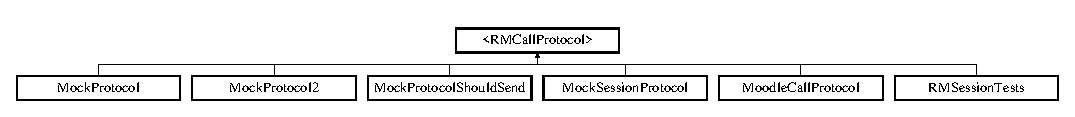
\includegraphics[height=1.3494cm]{protocol_r_m_call_protocol-p}
\end{center}
\end{figure}
\subsection*{Public Member Functions}
\begin{DoxyCompactItemize}
\item 
(BOOL) -\/ \hyperlink{protocol_r_m_call_protocol-p_a5656dcb18011d94f1d2de1e695741279}{requestShouldSend:method:arguments:}
\begin{DoxyCompactList}\small\item\em Should the request be sent? \item\end{DoxyCompactList}\item 
(void) -\/ \hyperlink{protocol_r_m_call_protocol-p_a33f653fd32cbeae77545d77d7d80575c}{requestWillSend:method:arguments:}
\begin{DoxyCompactList}\small\item\em An event fired just before the request is sent. \item\end{DoxyCompactList}\item 
(void) -\/ \hyperlink{protocol_r_m_call_protocol-p_ae502b8d3070e9de7a6b125b16a8db5cf}{requestDidSend:method:arguments:}
\begin{DoxyCompactList}\small\item\em An event fired just after the request is sent. \item\end{DoxyCompactList}\item 
(void) -\/ \hyperlink{protocol_r_m_call_protocol-p_ab3c27370fb06c6083131b5338dcabe2f}{adjustRequest:method:arguments:}
\begin{DoxyCompactList}\small\item\em Adjust the request object according to this call protocol. \item\end{DoxyCompactList}\item 
(BOOL) -\/ \hyperlink{protocol_r_m_call_protocol-p_ae4432e31198f1f116480ec4f1ed46d92}{isAsynchronous}
\begin{DoxyCompactList}\small\item\em Whether the call protocol is asynchronous. \item\end{DoxyCompactList}\end{DoxyCompactItemize}


\subsection{Detailed Description}
Provides call protocol interface/implementation. 

Definition at line 17 of file RMCall.h.

\subsection{Member Function Documentation}
\hypertarget{protocol_r_m_call_protocol-p_a5656dcb18011d94f1d2de1e695741279}{
\index{RMCallProtocol-\/p@{RMCallProtocol-\/p}!requestShouldSend:method:arguments:@{requestShouldSend:method:arguments:}}
\index{requestShouldSend:method:arguments:@{requestShouldSend:method:arguments:}!RMCallProtocol-p@{RMCallProtocol-\/p}}
\subsubsection[{requestShouldSend:method:arguments:}]{\setlength{\rightskip}{0pt plus 5cm}-\/ (BOOL) requestShouldSend: (ASIFormDataRequest $\ast$) {\em request}\/ method: (NSString $\ast$) {\em method}\/ arguments: (NSDictionary $\ast$) {\em arguments}\hspace{0.3cm}{\ttfamily  \mbox{[}optional\mbox{]}}}}
\label{protocol_r_m_call_protocol-p_a5656dcb18011d94f1d2de1e695741279}


Should the request be sent? 
\begin{DoxyParams}{Parameters}
\item[{\em request}]The request object. \item[{\em method}]The method name. \item[{\em arguments}]The arguments for the call.\end{DoxyParams}
\begin{DoxyReturn}{Returns}
Whether this request should be sent. 
\end{DoxyReturn}
\hypertarget{protocol_r_m_call_protocol-p_a33f653fd32cbeae77545d77d7d80575c}{
\index{RMCallProtocol-\/p@{RMCallProtocol-\/p}!requestWillSend:method:arguments:@{requestWillSend:method:arguments:}}
\index{requestWillSend:method:arguments:@{requestWillSend:method:arguments:}!RMCallProtocol-p@{RMCallProtocol-\/p}}
\subsubsection[{requestWillSend:method:arguments:}]{\setlength{\rightskip}{0pt plus 5cm}-\/ (void) requestWillSend: (ASIFormDataRequest $\ast$) {\em request}\/ method: (NSString $\ast$) {\em method}\/ arguments: (NSDictionary $\ast$) {\em arguments}\hspace{0.3cm}{\ttfamily  \mbox{[}optional\mbox{]}}}}
\label{protocol_r_m_call_protocol-p_a33f653fd32cbeae77545d77d7d80575c}


An event fired just before the request is sent. 
\begin{DoxyParams}{Parameters}
\item[{\em request}]The request object. \item[{\em method}]The method name. \item[{\em arguments}]The arguments for the call. \end{DoxyParams}
\hypertarget{protocol_r_m_call_protocol-p_ae502b8d3070e9de7a6b125b16a8db5cf}{
\index{RMCallProtocol-\/p@{RMCallProtocol-\/p}!requestDidSend:method:arguments:@{requestDidSend:method:arguments:}}
\index{requestDidSend:method:arguments:@{requestDidSend:method:arguments:}!RMCallProtocol-p@{RMCallProtocol-\/p}}
\subsubsection[{requestDidSend:method:arguments:}]{\setlength{\rightskip}{0pt plus 5cm}-\/ (void) requestDidSend: (ASIFormDataRequest $\ast$) {\em request}\/ method: (NSString $\ast$) {\em method}\/ arguments: (NSDictionary $\ast$) {\em arguments}\hspace{0.3cm}{\ttfamily  \mbox{[}optional\mbox{]}}}}
\label{protocol_r_m_call_protocol-p_ae502b8d3070e9de7a6b125b16a8db5cf}


An event fired just after the request is sent. 
\begin{DoxyParams}{Parameters}
\item[{\em request}]The request object. \item[{\em method}]The method name. \item[{\em arguments}]The arguments for the call. \end{DoxyParams}
\hypertarget{protocol_r_m_call_protocol-p_ab3c27370fb06c6083131b5338dcabe2f}{
\index{RMCallProtocol-\/p@{RMCallProtocol-\/p}!adjustRequest:method:arguments:@{adjustRequest:method:arguments:}}
\index{adjustRequest:method:arguments:@{adjustRequest:method:arguments:}!RMCallProtocol-p@{RMCallProtocol-\/p}}
\subsubsection[{adjustRequest:method:arguments:}]{\setlength{\rightskip}{0pt plus 5cm}-\/ (void) adjustRequest: (ASIFormDataRequest $\ast$) {\em request}\/ method: (NSString $\ast$) {\em method}\/ arguments: (NSDictionary $\ast$) {\em arguments}\hspace{0.3cm}{\ttfamily  \mbox{[}required\mbox{]}}}}
\label{protocol_r_m_call_protocol-p_ab3c27370fb06c6083131b5338dcabe2f}


Adjust the request object according to this call protocol. 
\begin{DoxyParams}{Parameters}
\item[{\em request}]The request object. \item[{\em method}]The method name. \item[{\em arguments}]The arguments for the call. \end{DoxyParams}
\hypertarget{protocol_r_m_call_protocol-p_ae4432e31198f1f116480ec4f1ed46d92}{
\index{RMCallProtocol-\/p@{RMCallProtocol-\/p}!isAsynchronous@{isAsynchronous}}
\index{isAsynchronous@{isAsynchronous}!RMCallProtocol-p@{RMCallProtocol-\/p}}
\subsubsection[{isAsynchronous}]{\setlength{\rightskip}{0pt plus 5cm}-\/ (BOOL) isAsynchronous \hspace{0.3cm}{\ttfamily  \mbox{[}optional\mbox{]}}}}
\label{protocol_r_m_call_protocol-p_ae4432e31198f1f116480ec4f1ed46d92}


Whether the call protocol is asynchronous. \begin{DoxyReturn}{Returns}
the call protocol is asynchronous or not, defaults to YES 
\end{DoxyReturn}


The documentation for this protocol was generated from the following file:\begin{DoxyCompactItemize}
\item 
/Users/yxh/Code/XCode/WIRemoting/Source/Classes/RMCall.h\end{DoxyCompactItemize}

\hypertarget{interface_r_m_call_tests}{
\section{RMCallTests Class Reference}
\label{interface_r_m_call_tests}\index{RMCallTests@{RMCallTests}}
}
\subsection*{Protected Attributes}
\begin{DoxyCompactItemize}
\item 
\hypertarget{interface_r_m_call_tests_a09775bdf02a3dd357630f87e2263a055}{
id {\bfseries protocol}}
\label{interface_r_m_call_tests_a09775bdf02a3dd357630f87e2263a055}

\item 
\hypertarget{interface_r_m_call_tests_acf178ef7ba187366a43cf708ba587051}{
\hyperlink{interface_r_m_call}{RMCall} $\ast$ {\bfseries call}}
\label{interface_r_m_call_tests_acf178ef7ba187366a43cf708ba587051}

\end{DoxyCompactItemize}


\subsection{Detailed Description}


Definition at line 21 of file RMCallTests.h.

The documentation for this class was generated from the following file:\begin{DoxyCompactItemize}
\item 
/Users/yxh/Code/XCode/WIRemoting/Tests/UnitTests/RMCallTests.h\end{DoxyCompactItemize}

\hypertarget{interface_r_m_response}{
\section{RMResponse Class Reference}
\label{interface_r_m_response}\index{RMResponse@{RMResponse}}
}


Handles call responses in WIRemoting framework.  


{\ttfamily \#import $<$RMResponse.h$>$}\subsection*{Public Member Functions}
\begin{DoxyCompactItemize}
\item 
\hypertarget{interface_r_m_response_a0f3e33e889c76f99c085b8a356dff03f}{
(id) -\/ {\bfseries initWithCall:request:delegate:}}
\label{interface_r_m_response_a0f3e33e889c76f99c085b8a356dff03f}

\item 
\hypertarget{interface_r_m_response_a9c0cb2ff676b85a95a880810222dc38e}{
(void) -\/ {\bfseries requestFinished:}}
\label{interface_r_m_response_a9c0cb2ff676b85a95a880810222dc38e}

\item 
\hypertarget{interface_r_m_response_a72bce836d142fbe400db06a9683e9d64}{
(void) -\/ {\bfseries requestFailed:}}
\label{interface_r_m_response_a72bce836d142fbe400db06a9683e9d64}

\item 
\hypertarget{interface_r_m_response_a647ba0ba05412d71c6cf8bd144b656ef}{
(NSString $\ast$) -\/ {\bfseries responseString}}
\label{interface_r_m_response_a647ba0ba05412d71c6cf8bd144b656ef}

\item 
\hypertarget{interface_r_m_response_a945e816c61e871826ef46689cd78d857}{
(NSData $\ast$) -\/ {\bfseries responseData}}
\label{interface_r_m_response_a945e816c61e871826ef46689cd78d857}

\end{DoxyCompactItemize}
\subsection*{Static Public Member Functions}
\begin{DoxyCompactItemize}
\item 
\hypertarget{interface_r_m_response_a6281bc247a32f1bda98b708eae184887}{
(id) + {\bfseries responseWithCall:request:delegate:}}
\label{interface_r_m_response_a6281bc247a32f1bda98b708eae184887}

\end{DoxyCompactItemize}
\subsection*{Protected Attributes}
\begin{DoxyCompactItemize}
\item 
\hypertarget{interface_r_m_response_aead684dffc01908a30b52a9fec734939}{
\hyperlink{interface_r_m_call}{RMCall} $\ast$ {\bfseries parentCall}}
\label{interface_r_m_response_aead684dffc01908a30b52a9fec734939}

\item 
\hypertarget{interface_r_m_response_a8e6cf0138d78a853f3d3d067a55e361a}{
NSArray $\ast$ {\bfseries delegateChain}}
\label{interface_r_m_response_a8e6cf0138d78a853f3d3d067a55e361a}

\item 
\hypertarget{interface_r_m_response_a8100e3ff4d7ad1ec1707c763a8690ff4}{
ASIHTTPRequest $\ast$ {\bfseries request}}
\label{interface_r_m_response_a8100e3ff4d7ad1ec1707c763a8690ff4}

\item 
\hypertarget{interface_r_m_response_a8a916fbec7712a005e611b7f5e4f4bdf}{
NSString $\ast$ {\bfseries string}}
\label{interface_r_m_response_a8a916fbec7712a005e611b7f5e4f4bdf}

\item 
\hypertarget{interface_r_m_response_a420513833840b50a963a6a1c2f02b975}{
NSData $\ast$ {\bfseries data}}
\label{interface_r_m_response_a420513833840b50a963a6a1c2f02b975}

\end{DoxyCompactItemize}


\subsection{Detailed Description}
Handles call responses in WIRemoting framework. 

Definition at line 18 of file RMResponse.h.

The documentation for this class was generated from the following files:\begin{DoxyCompactItemize}
\item 
/Users/yxh/Code/XCode/WIRemoting/Source/Classes/RMResponse.h\item 
/Users/yxh/Code/XCode/WIRemoting/Source/Classes/RMResponse.m\end{DoxyCompactItemize}

\hypertarget{protocol_r_m_result_delegate-p}{
\section{$<$RMResultDelegate$>$ Protocol Reference}
\label{protocol_r_m_result_delegate-p}\index{RMResultDelegate-\/p@{RMResultDelegate-\/p}}
}


Handles call results in WIRemoting framework.  


{\ttfamily \#import $<$RMCall.h$>$}Inheritance diagram for $<$RMResultDelegate$>$::\begin{figure}[H]
\begin{center}
\leavevmode
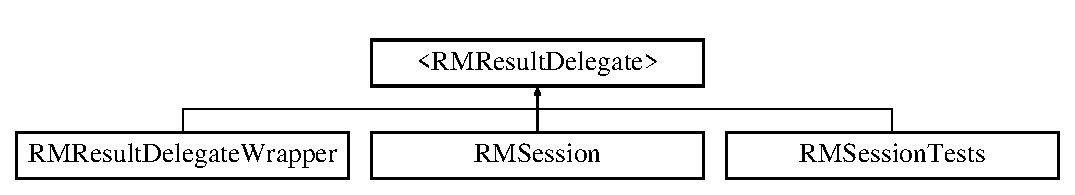
\includegraphics[height=2cm]{protocol_r_m_result_delegate-p}
\end{center}
\end{figure}
\subsection*{Public Member Functions}
\begin{DoxyCompactItemize}
\item 
(void) -\/ \hyperlink{protocol_r_m_result_delegate-p_a965fe7cc4e150bb6ecf7cbb02b9c7248}{finished:}
\begin{DoxyCompactList}\small\item\em An event fired when the call successfully finishes. \item\end{DoxyCompactList}\item 
(void) -\/ \hyperlink{protocol_r_m_result_delegate-p_a3521cd9555449b32aabdb759d2dadce5}{failed:error:}
\begin{DoxyCompactList}\small\item\em An event fired when the call fails. \item\end{DoxyCompactList}\end{DoxyCompactItemize}


\subsection{Detailed Description}
Handles call results in WIRemoting framework. 

Definition at line 82 of file RMCall.h.

\subsection{Member Function Documentation}
\hypertarget{protocol_r_m_result_delegate-p_a965fe7cc4e150bb6ecf7cbb02b9c7248}{
\index{RMResultDelegate-\/p@{RMResultDelegate-\/p}!finished:@{finished:}}
\index{finished:@{finished:}!RMResultDelegate-p@{RMResultDelegate-\/p}}
\subsubsection[{finished:}]{\setlength{\rightskip}{0pt plus 5cm}-\/ (void) finished: ({\bf RMResponse} $\ast$) {\em response}\hspace{0.3cm}{\ttfamily  \mbox{[}required\mbox{]}}}}
\label{protocol_r_m_result_delegate-p_a965fe7cc4e150bb6ecf7cbb02b9c7248}


An event fired when the call successfully finishes. 
\begin{DoxyParams}{Parameters}
\item[{\em response}]A response object from the remote call. \end{DoxyParams}


Reimplemented in \hyperlink{interface_mock_ab15e59579bf7b5c5de900d28374062b7}{Mock}.\hypertarget{protocol_r_m_result_delegate-p_a3521cd9555449b32aabdb759d2dadce5}{
\index{RMResultDelegate-\/p@{RMResultDelegate-\/p}!failed:error:@{failed:error:}}
\index{failed:error:@{failed:error:}!RMResultDelegate-p@{RMResultDelegate-\/p}}
\subsubsection[{failed:error:}]{\setlength{\rightskip}{0pt plus 5cm}-\/ (void) failed: ({\bf RMResponse} $\ast$) {\em response}\/ error: (NSError $\ast$) {\em error}\hspace{0.3cm}{\ttfamily  \mbox{[}required\mbox{]}}}}
\label{protocol_r_m_result_delegate-p_a3521cd9555449b32aabdb759d2dadce5}


An event fired when the call fails. 
\begin{DoxyParams}{Parameters}
\item[{\em response}]A response object from the remote peer. \item[{\em error}]An error object from the remote peer. \end{DoxyParams}


Reimplemented in \hyperlink{interface_mock_ae57e780c8ddcf5c4c79af12c54d58cff}{Mock}.

The documentation for this protocol was generated from the following file:\begin{DoxyCompactItemize}
\item 
/Users/yxh/Code/XCode/WIRemoting/Source/Classes/RMCall.h\end{DoxyCompactItemize}

\hypertarget{interface_r_m_session}{
\section{RMSession Class Reference}
\label{interface_r_m_session}\index{RMSession@{RMSession}}
}


Handles sessions in WIRemoting framework.  


{\ttfamily \#import $<$RMSession.h$>$}Inheritance diagram for RMSession::\begin{figure}[H]
\begin{center}
\leavevmode
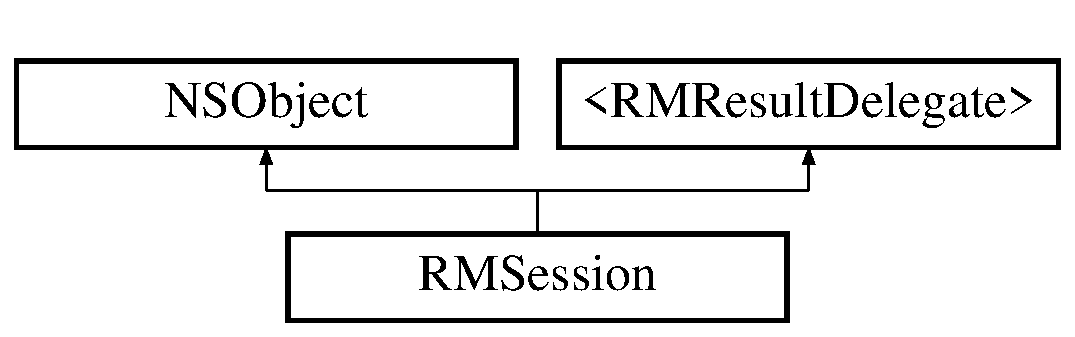
\includegraphics[height=2cm]{interface_r_m_session}
\end{center}
\end{figure}
\subsection*{Public Member Functions}
\begin{DoxyCompactItemize}
\item 
(id) -\/ \hyperlink{interface_r_m_session_ac0cd1eaf70a3afee073b376773d915ff}{initWithAuthenticator:call:delegate:}
\begin{DoxyCompactList}\small\item\em Initiate a session with an authentication delegate. \item\end{DoxyCompactList}\item 
\hypertarget{interface_r_m_session_aba47598cf422661784044b0f24286939}{
(void) -\/ \hyperlink{interface_r_m_session_aba47598cf422661784044b0f24286939}{authenticate}}
\label{interface_r_m_session_aba47598cf422661784044b0f24286939}

\begin{DoxyCompactList}\small\item\em Authenticate the session. \item\end{DoxyCompactList}\item 
(BOOL) -\/ \hyperlink{interface_r_m_session_a898ba9b048b6568b051acde8d2f48749}{call:arguments:delegate:}
\begin{DoxyCompactList}\small\item\em Call a method. \item\end{DoxyCompactList}\item 
\hypertarget{interface_r_m_session_a77c806e25987046026c7bb60accabe1b}{
(void) -\/ \hyperlink{interface_r_m_session_a77c806e25987046026c7bb60accabe1b}{close}}
\label{interface_r_m_session_a77c806e25987046026c7bb60accabe1b}

\begin{DoxyCompactList}\small\item\em Close a session. \item\end{DoxyCompactList}\end{DoxyCompactItemize}
\subsection*{Protected Attributes}
\begin{DoxyCompactItemize}
\item 
\hypertarget{interface_r_m_session_a759f830479707308f14b1405f6968379}{
id$<$ \hyperlink{protocol_r_m_authenticator-p}{RMAuthenticator} $>$ {\bfseries authenticator}}
\label{interface_r_m_session_a759f830479707308f14b1405f6968379}

\end{DoxyCompactItemize}
\subsection*{Properties}
\begin{DoxyCompactItemize}
\item 
\hypertarget{interface_r_m_session_a1eb4cd25fd5ff4adb90fd2025b2bd3ee}{
\hyperlink{interface_r_m_call}{RMCall} $\ast$ \hyperlink{interface_r_m_session_a1eb4cd25fd5ff4adb90fd2025b2bd3ee}{call}}
\label{interface_r_m_session_a1eb4cd25fd5ff4adb90fd2025b2bd3ee}

\begin{DoxyCompactList}\small\item\em The call object to handle session calls. \item\end{DoxyCompactList}\item 
\hypertarget{interface_r_m_session_a9f50b3e61cc57115a00bddcecf64f793}{
id$<$ \hyperlink{protocol_r_m_result_delegate-p}{RMResultDelegate} $>$ \hyperlink{interface_r_m_session_a9f50b3e61cc57115a00bddcecf64f793}{delegate}}
\label{interface_r_m_session_a9f50b3e61cc57115a00bddcecf64f793}

\begin{DoxyCompactList}\small\item\em The session delegate to handle authentication events. \item\end{DoxyCompactList}\item 
BOOL \hyperlink{interface_r_m_session_a71acbe4da4033e724b01e44d39ea2f24}{authenticated}
\begin{DoxyCompactList}\small\item\em Return the state whether the session is authenticated. \item\end{DoxyCompactList}\end{DoxyCompactItemize}


\subsection{Detailed Description}
Handles sessions in WIRemoting framework. 

Definition at line 63 of file RMSession.h.

\subsection{Member Function Documentation}
\hypertarget{interface_r_m_session_ac0cd1eaf70a3afee073b376773d915ff}{
\index{RMSession@{RMSession}!initWithAuthenticator:call:delegate:@{initWithAuthenticator:call:delegate:}}
\index{initWithAuthenticator:call:delegate:@{initWithAuthenticator:call:delegate:}!RMSession@{RMSession}}
\subsubsection[{initWithAuthenticator:call:delegate:}]{\setlength{\rightskip}{0pt plus 5cm}-\/ (id) initWithAuthenticator: (id$<${\bf RMAuthenticator}$>$) {\em authenticator}\/ call: ({\bf RMCall}$\ast$) {\em call}\/ delegate: (id$<${\bf RMResultDelegate}$>$) {\em delegate}}}
\label{interface_r_m_session_ac0cd1eaf70a3afee073b376773d915ff}


Initiate a session with an authentication delegate. 
\begin{DoxyParams}{Parameters}
\item[{\em authenticator}]An authentication service provider. \item[{\em call}]A call object to handle session calls. \item[{\em delegate}]A session delegate to handle authentication events.\end{DoxyParams}
\begin{DoxyReturn}{Returns}
An initiated \hyperlink{interface_r_m_session}{RMSession} object. 
\end{DoxyReturn}


Definition at line 17 of file RMSession.m.\hypertarget{interface_r_m_session_a898ba9b048b6568b051acde8d2f48749}{
\index{RMSession@{RMSession}!call:arguments:delegate:@{call:arguments:delegate:}}
\index{call:arguments:delegate:@{call:arguments:delegate:}!RMSession@{RMSession}}
\subsubsection[{call:arguments:delegate:}]{\setlength{\rightskip}{0pt plus 5cm}-\/ (BOOL) call: (NSString$\ast$) {\em method}\/ arguments: (NSDictionary$\ast$) {\em arguments}\/ delegate: (id$<${\bf RMResultDelegate}$>$) {\em delegate}}}
\label{interface_r_m_session_a898ba9b048b6568b051acde8d2f48749}


Call a method. 
\begin{DoxyParams}{Parameters}
\item[{\em method}]The method name. \item[{\em arguments}]Method arguments. \item[{\em delegate}]The call delegate to handle call results. \end{DoxyParams}


Definition at line 99 of file RMSession.m.

\subsection{Property Documentation}
\hypertarget{interface_r_m_session_a71acbe4da4033e724b01e44d39ea2f24}{
\index{RMSession@{RMSession}!authenticated@{authenticated}}
\index{authenticated@{authenticated}!RMSession@{RMSession}}
\subsubsection[{authenticated}]{\setlength{\rightskip}{0pt plus 5cm}-\/ (BOOL) authenticated\hspace{0.3cm}{\ttfamily  \mbox{[}read, assign\mbox{]}}}}
\label{interface_r_m_session_a71acbe4da4033e724b01e44d39ea2f24}


Return the state whether the session is authenticated. \begin{DoxyReturn}{Returns}
whether the session is authenticated. 
\end{DoxyReturn}


Definition at line 67 of file RMSession.h.

The documentation for this class was generated from the following files:\begin{DoxyCompactItemize}
\item 
/Users/yxh/Code/XCode/WIRemoting/Source/Classes/RMSession.h\item 
/Users/yxh/Code/XCode/WIRemoting/Source/Classes/RMSession.m\end{DoxyCompactItemize}

\hypertarget{interface_r_m_session_tests}{
\section{RMSessionTests Class Reference}
\label{interface_r_m_session_tests}\index{RMSessionTests@{RMSessionTests}}
}
Inheritance diagram for RMSessionTests::\begin{figure}[H]
\begin{center}
\leavevmode
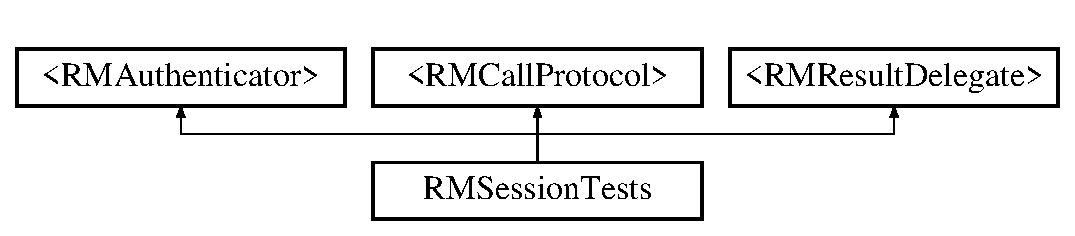
\includegraphics[height=2cm]{interface_r_m_session_tests}
\end{center}
\end{figure}
\subsection*{Protected Attributes}
\begin{DoxyCompactItemize}
\item 
\hypertarget{interface_r_m_session_tests_abeeb4a2ae56b6847a234db1299576652}{
\hyperlink{interface_r_m_call}{RMCall} $\ast$ {\bfseries call}}
\label{interface_r_m_session_tests_abeeb4a2ae56b6847a234db1299576652}

\item 
\hypertarget{interface_r_m_session_tests_a15addac7538f41a12439e0babefa8935}{
\hyperlink{interface_r_m_session}{RMSession} $\ast$ {\bfseries session}}
\label{interface_r_m_session_tests_a15addac7538f41a12439e0babefa8935}

\item 
\hypertarget{interface_r_m_session_tests_a4033c142c7ba3bef1d359ef19b4382a7}{
\hyperlink{interface_mock_protocol}{MockProtocol} $\ast$ {\bfseries protocol}}
\label{interface_r_m_session_tests_a4033c142c7ba3bef1d359ef19b4382a7}

\item 
\hypertarget{interface_r_m_session_tests_ada7aafce83843a941668b5d0f83c9ad3}{
NSString $\ast$ {\bfseries username}}
\label{interface_r_m_session_tests_ada7aafce83843a941668b5d0f83c9ad3}

\item 
\hypertarget{interface_r_m_session_tests_a5b3ca57860668a61e67ded4d00a0eac5}{
NSString $\ast$ {\bfseries password}}
\label{interface_r_m_session_tests_a5b3ca57860668a61e67ded4d00a0eac5}

\end{DoxyCompactItemize}


\subsection{Detailed Description}


Definition at line 22 of file RMSessionTests.h.

The documentation for this class was generated from the following file:\begin{DoxyCompactItemize}
\item 
/Users/yxh/Code/XCode/WIRemoting/Source/Tests/UnitTests/RMSessionTests.h\end{DoxyCompactItemize}

\hypertarget{interface_r_m_status}{
\section{RMStatus Class Reference}
\label{interface_r_m_status}\index{RMStatus@{RMStatus}}
}
Inheritance diagram for RMStatus::\begin{figure}[H]
\begin{center}
\leavevmode
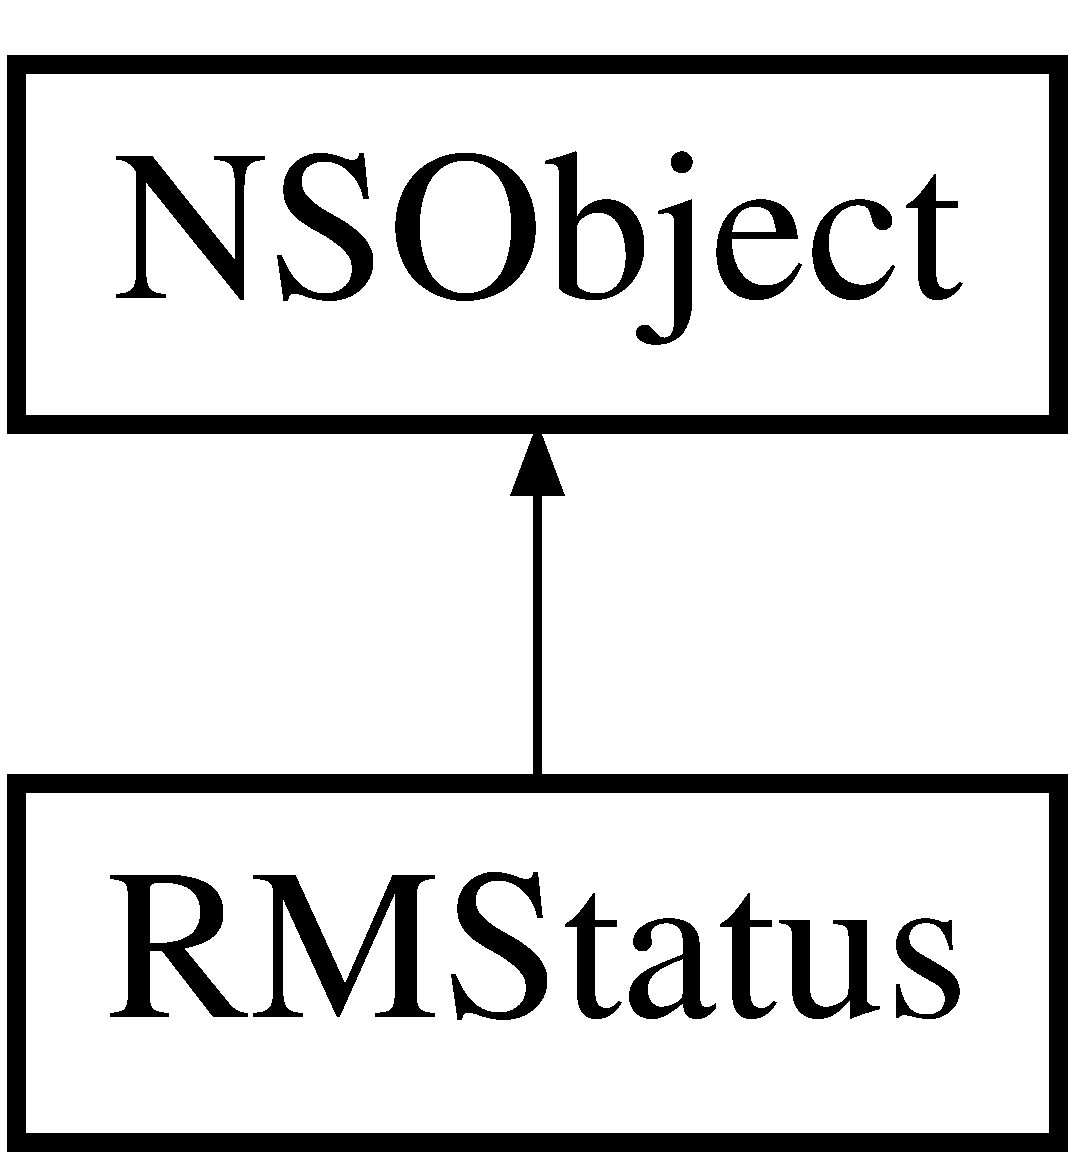
\includegraphics[height=2cm]{interface_r_m_status}
\end{center}
\end{figure}


\subsection{Detailed Description}


Definition at line 12 of file RMStatus.h.

The documentation for this class was generated from the following file:\begin{DoxyCompactItemize}
\item 
/Users/yxh/Code/XCode/WIRemoting/Classes/RMStatus.h\end{DoxyCompactItemize}

\printindex
\end{document}
